\documentclass{article} % For LaTeX2e
\usepackage{nips12submit_e,times,amsmath,hyperref}
%\documentstyle[nips12submit_09,times,art10]{article} % For LaTeX 2.09
\usepackage{graphicx}


\title{Molecular Mechanics Force Field Optimization}


\author{
Subhodeep Moitra\\
Language Technologies Institute\\
\texttt{subhodee@andrew.cmu.edu} \\
\And
Chunlei Liu \\
Physics Department \\
\texttt{chl56@andrew.cmu.edu} 
}
\newcommand{\fix}{\marginpar{FIX}}
\newcommand{\new}{\marginpar{NEW}}

\nipsfinalcopy % Uncomment for camera-ready version

\begin{document}


\maketitle

\section{Introduction}
In this project we propose to study and optimize molecular mechanics energy functions. Each biological macromolecule has an associated energy function which determines its shape and stability. This energy function E is normally defined in terms of the biophysical properties of the atoms in the macromolecule. E is also related to the three dimensional shape taken by the biological macromolecule. E encompasses electrostatic calculations, van der waals forces and even explicit modelling of the hydrogen bonds \cite{Boas2007}. The macromolecule can assume a number of different conformations or shapes which gives rise to different energy values. The natively occurring conformation is the one that is most stable and also has the lowest energy E*. Finding the global minima of this function is referred to as the \emph{Protein Folding problem}. Minimizing this function is very hard as E has a rugged landscape. This problem is one of the hardest problems facing science today and the solution of which which can lead to many biomedical breakthroughs. 

We first examine in detail the terms in the energy function that make the optimization problem hard. We also present a brief review on some commonly used methods such as conjugate gradient descent which can be used to approximately solve the optimization problem. We  then proceed to show how certain assumptions made about the protein backbone(defined in next section), state space and the form of the energy function can be used to simplify the problem and pose it as an Integer Linear Program(ILP). We attempt to solve a simplified version of the problem called the \emph{Side Chain Prediction problem} \cite{review_paper}. We show connections of the ILP to branch and bound methods such as DEE and A*. We also comment on the conditions under which an IP relaxed to an  LP gives rise to naturally integer solutions. 

\section{Protein Stucture}
One important application of energy minimization is to study the protein structure. The structural hierarchy of the protein can
 be divided into primary structure, secondary structure, tertiary structure and quaternary structure following the order\cite{protein}. 
The primary structure in a protein refers to the set of chemical bonds which can be simply denoted as the amino acid sequence. 
It is known that more than 10 thousands proteins in our body are just composed of different arrangements of 20 types of amino acid
residues. Each amino acid consists of a backbone part which is common to all the amino acid types, and a side chain part which is
unique to itself.  The secondary structure of a protein refers to those highly regular local sub-structures, which are mainly defined
by distributions of helices and strands. Two main types of these secondary structure are called the alpha helix and beta strands.
The tertiary structure of a protein is defined by the spatial assembly and interactions of the helices and strands. In this case,
the alpha helices and beta strands are folded into a compact globule, which is driven by the non-specific hydrophobic interactions.
The quaternary structure of a protein is composed of more than one subunit protein, which is stabilized by the same non-covalent 
interactions of disulfide bonds as the tertiary structure.

\section{Complexity of the potential energy function}

As previously described, the potential energy function of a protein consists of two main parts: the bonded part and the non-bonded part.
The bonded part includes the bound length term, the bound angle term, and the torsion angle terms. The non-bonded part includes the 
Lennard-Jones or Vander Waals term, and the Coulomb or electrostatic term. The typical shape of each individual term of the energy functions
is shown in Fig.~\ref{fig:energy}. As one can see from this figure, the terms for the bond length and bond angle are basically quadratic functions,
which are convex and easy to optimize. There are  reasons for this based on chemistry. When two atoms are connected by a chemical bond, they 
tend to maintain a fixed distance. Similar to the bond length, when three atoms are connected through two chemical bonds, the two bonds
tend to form a fixed angle.  The dihedral angle potential describes the interaction arising from torsional forces in molecules.
The corresponding term for the dihedral angle is periodic as shown in the plot. Although it is not convex, if we constrain the range in one
period, it should be easy to find the minimum. The Lennard-Jones term models the interaction of a pair of neutral atoms or molecules, which is 
attractive if they are far away and repulsive if they are too close. This term is not convex, but the minimum might be easy to find depending 
on deep it is.  The last term represents the electrostatic forces between charged atoms, which has minimum at zero or infinity distance 
depending on their charges. 


\begin{figure}[h!] 
\begin{center} 
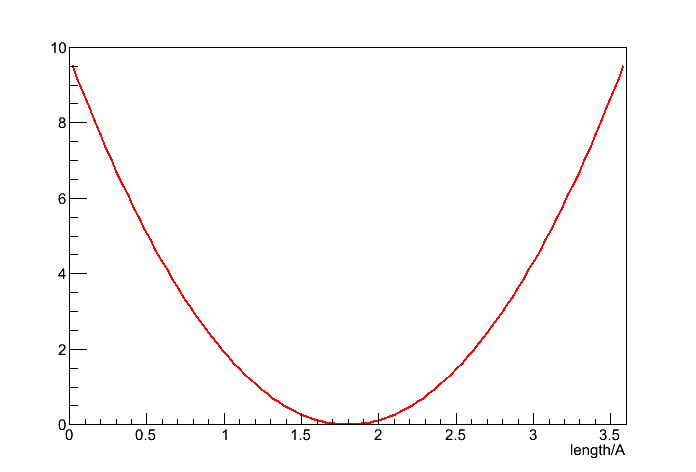
\includegraphics[width=0.4\textwidth]{bond.png}
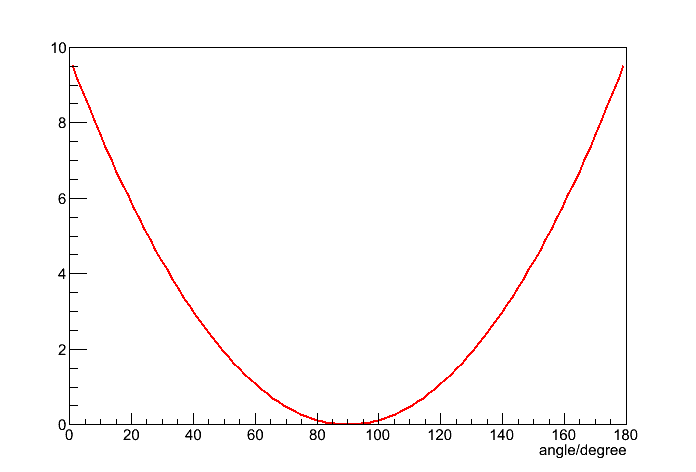
\includegraphics[width=0.4\textwidth]{angle.png}
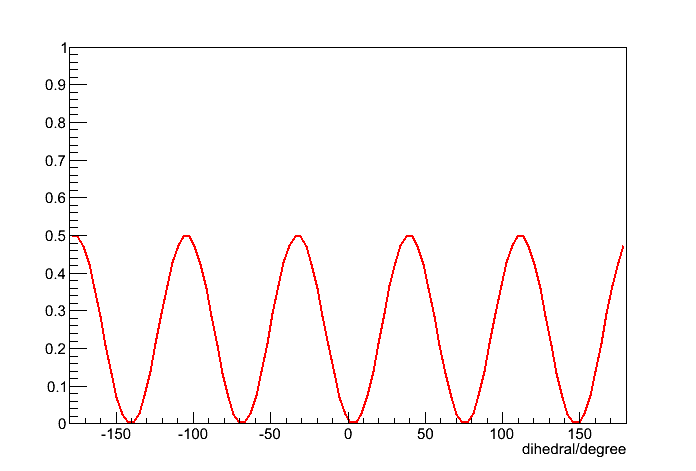
\includegraphics[width=0.4\textwidth]{dihedral.png}
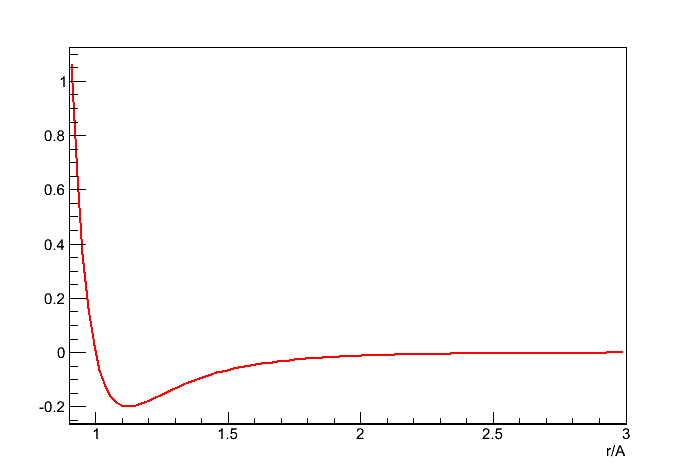
\includegraphics[width=0.4\textwidth]{pair.png}
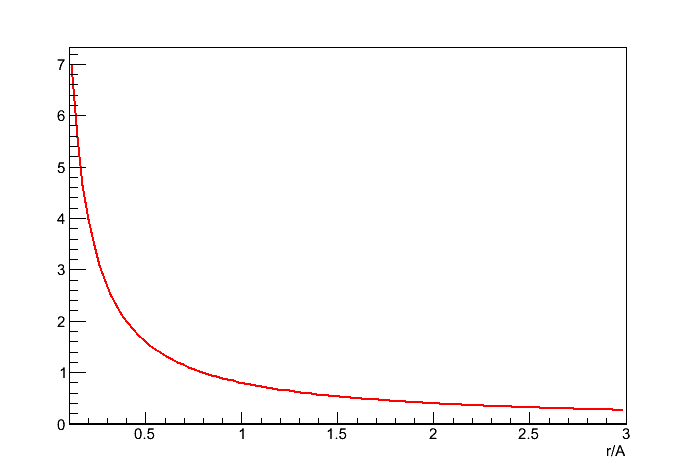
\includegraphics[width=0.4\textwidth]{pair2.png}
\end{center}  
\caption{ (top left):the bond terms as $\sum_{bonds} K_b(r-r_0)^2$, (top right): the angle term as $\sum_{angles} K_{\theta}(\theta-\theta_0)^2$,
(middle left): the torsion angle term as $\sum_{dihedral} K_{\phi}(1-\cos(n\phi-\delta))$,(middle right):the Lennard-Jones term as $\sum_{pairs} (\frac{A_{ij}}{r^{12}_{ij}}-\frac{B_{ij}}{r^{6}_{ij}})$,
(bottom):the Coulomb term as $\sum_{bonds} \frac{q_iq_j}{\epsilon r_{ij}}$}
\label{fig:energy}
\end{figure} 

\pagebreak

In practice, the bond length and bond angle terms are very stable and can be considered as fixed in the global
minimization. If there are no angles or dihedral angles involved in this minimization, the problem would be much easier to solve.
For a system of $n$ atoms, there are $n(n-1)/2$ pairs in total, and one can minimization the function for each pair individually.
However the existence of angles and dihedral angles make things not independent anymore. Take a system of 4 atoms as an example as 
shown in Fig.~\ref{fig:3d}, where the distance between atom 1 and atom 3 $r_{13}$ is related with $r_{12} $ and $r_{23}$ through 
bond angle $\theta$: $r_{13}=\sqrt{r^2_{12}+r^2_{23}-2r_{12}r_{23}\cos(\theta)}$. The relation between dihedral angle $\phi$ and 
distance between atoms and their direction is even more complex as: 
$\phi=\mbox{atan2}( r_{23}\vec{r}_{12}\cdot[\vec{r}_{23}\times\vec{r}_{34}], [\vec{r}_{12}\times\vec{r}_{23}]\cdot [\vec{r}_{23}\times\vec{r}_{34}] )$.



\begin{figure} 
\begin{center} 
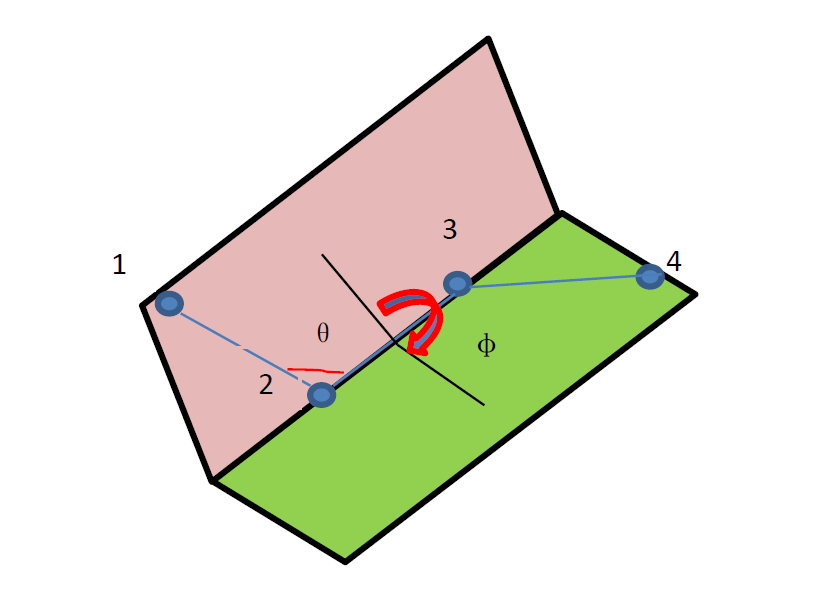
\includegraphics[width=0.5\textwidth]{3dangle.png}
\end{center}  
\caption{Bond angle and dihedral angle in a system of 4 atoms. }
\label{fig:3d}
\end{figure} 

\section{Minimization Methods}
As discussed above, the potential energy function is complex, rugged and non-convex, so finding the global minimum is hard. Several methods or algorithms
can be used to obtain the local minimum on the other hand. The first obvious method is to use the steepest descent method. Basically we move 
along the direction of the the gradient of the energy function at each step, and adjust the step-size such that we decrease the function value at most.
This method works very well if the gradient is large, but might have poor convergence when the gradient becomes smaller as a minimum is approached.
The second method we can use is the conjugate gradient method. In this method, the gradient calculated from previous steps are stored, and a new
conjugate direction is chosen for each new step. By doing this, it generally finds a minimum in a fewer steps than the steepest descent method as it
avoids the zig-zag pattern introduced in the steepest descent method. The third method is the Newton-Raphson method. By approximating the function as 
a quadratic term at each iteration, it predicts the location of a minimum and heads in that direction. The second derivatives are calculated or approximated
using the BFGS method. Thus extra storage might require substantial amounts of computer memory.  The Newton-Raphson method is expected to find
 the local minimum faster than the gradient-only methods. For all these methods mentioned above, bad initial conformation which is far from a
minimum can cause problems, which is especially serious for the Newton-Raphson method.


In the following we show the specific conjugate gradient algorithm which could be applied in our energy minimization problem~\cite{conjucate}. 
\begin{itemize}
\item 1. \texttt{Start with initial point $\vec{r}_0$, set $i=0, E_0=E(\vec{r}_0), \vec{x}_0 = -\nabla E(\vec{r}_0), \vec{g}_0=\vec{x}_0, \vec{h}_0=\vec{x}_0$  }
\item 2. \texttt{Minimize $E(\vec{r}_i+\alpha \vec{x}_i)$ with respect to scalar $\alpha$, set $\vec{r}_{i+1}= \vec{r}_i +\alpha \vec{x}_i$, get $E_{i+1}= E(\vec{r}_{i+1})$ }
\item 3. \texttt{if $|E_{i+1} - E_{i}| < \epsilon$, quit }
\item 4. \texttt{Calculate $\vec{x}_i=\nabla E(\vec{r}_{i+1})$ , and set $E_i=E_{i+1}$}
\item 5. \texttt{Calculate $\gamma = (\vec{x}_i\cdot \vec{x}_i)/(\vec{g}_i\cdot \vec{g}_i)$  }
\item 6. \texttt{Set $\vec{g}_{i+1} = \vec{x}_i$}
\item 7. \texttt{Set $\vec{h}_{i+1} = \vec{g}_{i+1} +\gamma \vec{h}_i$ and $\vec{x}_{i+1} =\vec{h}_{i+1}$}
\item 8. \texttt{Set $i=i+1$ and return to step 2 } 
\end{itemize}

\section{Simplification to Side Chain Optimization Problem}
As illustrated in the previous sections, the form of the energy terms are hard to optimize. An example of this is the Lennard Jones potential $\sum_{pairs} (\frac{A_{ij}}{r^{12}_{ij}}-\frac{B_{ij}}{r^{6}_{ij}})$. We explored ways in which the problem can be suitably modified so as to make the problem more tractable. 

In summary we made the following simplifying assumptions :
\begin{itemize}
\item Fixed backbone but flexible side chains
\item Discretize side chain chain angles 
\item Pairwise energy functions
\end{itemize}

The problem can then be stated as : 





\section{Integer Programming Formulation}
Read Review paper

\section{Relationship to DEE and A*}
Read review paper

\section{Relaxations to Linear Programming Formulation}
Read review paper

\section{Next Steps}


\begin{thebibliography}{99}

\bibitem{protein}
Pauling L, Corey RB, Branson HR (1951). "The structure of proteins; 
two hydrogen-bonded helical configurations of the polypeptide chain". Proc Natl Acad Sci USA 37 (4): 205211. 
doi:10.1073\/pnas.37.4.205. PMC 1063337. PMID 14816373

\bibitem{conjucate}
N. Andrei, “Conjugate Gradient Algorithms for Molecular Formation Under
Pairwise Potential Minimization,” Optimization, 2007.


\end{thebibliography}



%\begin{thebibliography}{9}
%
%\bibitem{BakerDas2008}
%	Das, R, Baker, D. 
%	\emph{Macromolecular modeling with rosetta},
%	Annu. Rev. Biochem., 77:363-82, 
%	2008.
%	
%\bibitem{Hetu2001}	
%	Kamisetty, H, Ramanathan, A, Bailey-Kellogg, C, Langmead, CJ ,
%	\emph{ Accounting for conformational entropy in predicting binding free energies of protein-protein interactions},
%	 Proteins, 79, 2:444-62,
%	2011
%
%\bibitem{Boas2007}
%	Boas, FE, Harbury, PB,
%	\emph{Potential energy functions for protein design},
%	Curr. Opin. Struct. Biol., 17, 2:199-204, 
%	2007
%	
%\end{thebibliography}
%

\end{document}
